\section{Сходимости случайных векторов}

Зафиксируем $\displaystyle \xi ,\{\xi _{n}\}_{n=1}^{\infty } -$случайные векторы.

\begin{definition}
	$\displaystyle \xi _{n}\xrightarrow{a.s.} \xi \xLeftrightarrow{Def} P\left( \xi _{n}\rightarrow \xi \right) =1\Leftrightarrow P\left(\left\{\omega :\xi _{n}( \omega )\rightarrow \xi ( \omega )\right\}\right) = 1$.
\end{definition}

\begin{exercise}
	Доказать, что $\displaystyle \left\{\omega :\xi _{n}( \omega )\rightarrow \xi ( \omega )\right\}$ -- измеримое множество.
\end{exercise}

\begin{definition}
	$\displaystyle \xi _{n}\xrightarrow{P} \xi \xLeftrightarrow{Def} \forall \varepsilon  >0\ P(\Vert \xi _{n} -\xi \Vert _{2}  >\varepsilon )\rightarrow 0$, где $\displaystyle \Vert x\Vert _{p} =\left(\sum _{i}| x_{i}| ^{p}\right)^{1/p}$.
\end{definition}

\begin{definition}
	$\displaystyle \xi _{n}\xrightarrow{L_{p}} \xi \xLeftrightarrow{Def} E(\Vert \xi _{n} -\xi \Vert _{p})^{p}\xrightarrow[n\rightarrow \infty ]{} 0$.
\end{definition}

\begin{exercise}
	Для чего обычно требуют $\displaystyle p\geqslant 1$?
\end{exercise}

\begin{definition}
	$\displaystyle \xi _{n}\xrightarrow{d} \xi \xLeftrightarrow{Def} \forall f:\mathbb{R}^{m}\rightarrow \mathbb{R}$ -- ограниченной и непрерывной выполняется $\displaystyle Ef( \xi _{n})\xrightarrow[n\rightarrow \infty ]{} Ef( \xi )$.
\end{definition}

\begin{exercise}
	Что будет если поменять непрерывность на равномерную непрерывность? А на липшицевость? (есть \href{https://arxiv.org/pdf/1610.05415.pdf}{здесь}, страница 41).
\end{exercise}

\begin{proposition}
	Пусть $\displaystyle \xi ,\{\xi _{n}\} \in \mathbb{R}^{m}$
	
	\begin{enumerate}
		\item $\displaystyle \xi _{n}\xrightarrow{a.s.} \xi \Leftrightarrow \forall i\in \overline{1,m} \ \xi _{n}^{( i)}\xrightarrow{a.s.} \xi ^{( i)}$
		
		\item $\displaystyle \xi _{n}\xrightarrow{P} \xi \Leftrightarrow \forall i\in \overline{1,m} \ \xi _{n}^{( i)}\xrightarrow{P} \xi ^{( i)}$
		
		\item $\displaystyle \xi _{n}\xrightarrow{L_{p}} \xi \Leftrightarrow \forall i\in \overline{1,m} \ \xi _{n}^{( i)}\xrightarrow{L_{p}} \xi ^{( i)}$
		
		\item $\displaystyle \xi _{n}\xrightarrow{d} \xi \Rightarrow \forall i\in \overline{1,m} \ \xi _{n}^{( i)}\xrightarrow{d} \xi ^{( i)}$
	\end{enumerate}
	
\end{proposition}

\begin{proof} ~
	\begin{enumerate}
		\item 
		\begin{gather*}
		    \left\{\xi _{n}\rightarrow \xi \right\} = \bigcap _{i=1}^{m}\left\{\xi _{n}^{( i)}\rightarrow \xi ^{( i)}\right\} \subset \left\{\xi _{n}^{( i)}\rightarrow \xi ^{( i)}\right\} \Rightarrow P\left( \xi _{n}\rightarrow \xi \right) \leqslant P\left( \xi _{n}^{( i)}\rightarrow \xi ^{( i)}\right) \ \forall i\in \overline{1,m}.
		\end{gather*}
		
		Пусть $\displaystyle \xi_n \xrightarrow{a.s.} \xi$. Тогда
		\begin{gather*}
		    1=P\left( \xi _{n}\rightarrow \xi \right) \leqslant P\left( \xi _{n}^{( i)}\rightarrow \xi ^{( i)}\right) \Rightarrow P\left( \xi _{n}^{( i)}\rightarrow \xi ^{( i)}\right) =1\ \forall i\in \overline{1,m}.
		\end{gather*}
		
		Обратно, пусть $\forall i\in \overline{1,m} \ \xi _{n}^{( i)}\xrightarrow{a.s.} \xi ^{( i)}$. Предположив противное, получаем
		\begin{gather*}
		    \{\xi _{n} \nrightarrow \xi \} = \bigcup _{i=1}^{m}\overline{\left\{\xi _{n}^{(i)}\rightarrow \xi ^{(i)}\right\}} =\bigcup _{i=1}^{m}\left\{\xi _{n}^{(i)} \nrightarrow \xi ^{(i)}\right\} \Rightarrow P( \xi _{n} \nrightarrow \xi ) \leqslant \sum _{i=1}^{m} P\left( \xi _{n}^{(i)} \nrightarrow \xi ^{(i)}\right) = 0.
		\end{gather*}
		
		\item Пусть $\xi _{n}\xrightarrow{P} \xi$, то есть
		\begin{gather*}
		    \displaystyle \forall \delta  >0\ \exists N:\forall n\geqslant N\ \delta  >P(\Vert \xi _{n} -\xi \Vert _{2}  >\varepsilon ).
		\end{gather*}
		Тогда
		\begin{gather*}
		    \delta  >P(\Vert \xi _{n} -\xi \Vert _{2}  >\varepsilon ) \geqslant P\left(\left| \xi _{n}^{( i)} -\xi ^{( i)}\right|  >\varepsilon \right) \geqslant 0\Rightarrow P\left(\left| \xi _{n}^{( i)} -\xi ^{( i)}\right|  >\varepsilon \right)\xrightarrow{n\rightarrow \infty } 0.
		\end{gather*}
		Обратно, пусть $\forall i\in \overline{1,m} \ \xi _{n}^{( i)}\xrightarrow{P} \xi ^{( i)}$. Тогда
		\begin{gather*}
		    \forall \varepsilon  >0\ \sqrt{\sum _{i=1}^{m}\left( \xi _{n}^{( i)} -\xi ^{( i)}\right)^{2}}  >\varepsilon \Leftrightarrow \sum _{i=1}^{m}\left( \xi _{n}^{( i)} -\xi ^{( i)}\right)^{2}  >\varepsilon ^{2} \Rightarrow \exists i:\left( \xi _{n}^{( i)} -\xi ^{( i)}\right)^{2}  >\frac{\varepsilon ^{2}}{m} \Leftrightarrow\\ \left| \xi _{n}^{( i)} -\xi ^{( i)}\right|  >\frac{\varepsilon }{\sqrt{m}}.
		\end{gather*}
		Получаем, что
		\begin{gather*}
		    P\left(\Vert \xi_n - \xi \Vert_2 > \varepsilon\right) \le \sum_{i=1}^m P\left(\left|\xi_n^{(i)} - \xi^{(i)}\right| > \frac{\varepsilon}{\sqrt{m}}\right) \xrightarrow{n\rightarrow\infty} 0.
		\end{gather*}
		
		\item
		\begin{gather*}
		    0\leqslant \left| \xi _{n}^{( i)} -\xi ^{( i)}\right| ^{p} \leqslant \sum _{i=1}^{m}\left| \xi _{n}^{( i)} -\xi ^{( i)}\right| ^{p}.
		\end{gather*}
		По свойству математического ожидания
		\begin{gather*}
		    0\leqslant E\left(\left| \xi _{n}^{( i)} -\xi ^{( i)}\right| ^{p}\right) \leqslant E\left(\sum _{i=1}^{m}\left| \xi _{n}^{( i)} -\xi ^{( i)}\right| ^{p}\right) \Rightarrow\\  E\left(\left|\xi_n^{(i)} - \xi^{(i)}\right|^p\right)^p \le E\left(\sum _{i=1}^{m}\left| \xi _{n}^{( i)} -\xi ^{( i)}\right| ^{p}\right)^p.
		\end{gather*}
		Пусть $\xi _{n}\xrightarrow{L_{p}} \xi$. Тогда
		\begin{gather*}
		    0 \le E\left(\left|\xi_n^{(i)} - \xi^{(i)}\right|^p\right)^p \le E\left(\sum _{i=1}^{m}\left| \xi _{n}^{( i)} -\xi ^{( i)}\right| ^{p}\right)^p \Rightarrow E\left(\left|\xi_n^{(i)} - \xi^{(i)}\right|^p\right)^p \xrightarrow{n\rightarrow\infty}0.
		\end{gather*}
		
		Обратно, пусть $\forall i\in \overline{1,m} \ \xi _{n}^{( i)}\xrightarrow{L_{p}} \xi ^{( i)}$. Тогда
		\begin{gather*}
		    \forall i \in \overline{1,m}\ E\left(\left|\xi_n^{(i)} - \xi^{(i)}\right|^p\right) \xrightarrow{n \rightarrow \infty} 0 \Rightarrow \sum_{i=1}^{m}E\left(\left|\xi_n^{(i)}- \xi^{(i)}\right|^p\right) \xrightarrow{n\rightarrow\infty} 0 \Rightarrow\\ E\left(\sum_{i=1}^{m}\left|\xi_n^{(i)}-\xi^{(i)}\right|^p\right)^p\xrightarrow{n\rightarrow\infty} 0.
		\end{gather*}
		
		\item Пусть $g:\R\rightarrow\R$ -- непрерывная ограниченная функция, $h:\R^m \rightarrow \R,\ h(x) = x^{(i)}$. Тогда $g \circ h$ -- непрерывная ограниченная функция и
		\begin{gather*}
		    E\left(g\left(\xi_n^{(i)}\right)\right) = E\left(g\left(h\left(\xi_n\right)\right)\right) \xrightarrow{n \rightarrow \infty} E\left(g\left(h\left(\xi\right)\right)\right) = E\left(g\left(\xi^{(i)}\right)\right).
		\end{gather*}
	\end{enumerate}

\end{proof}

\begin{exercise}
	Показать, что в п.4 обратная импликация неверна.
\end{exercise}

\begin{proposition}
	Пусть $\left\{\xi_n\right\}_{n=1}^\infty$ -- случайные векторы, и $\xi_n \xrightarrow{d} c = const$, то $\xi_n \xrightarrow{P} c$.
\end{proposition}

\begin{proof}
	Из п.4 предыдущего утверждения
	\begin{gather*}
	    \forall i \in \overline{1,m}\ \xi_n^{(i)} \xrightarrow{d} c^{(i)} \Rightarrow \xi_n^{(i)} \xrightarrow{P} c^{(i)} \xRightarrow[]{p.2} \xi_n \xrightarrow{P} c.
	\end{gather*}
\end{proof}

\begin{theorem}
	(б/д) 
	Пусть $\xi,\ \left\{\xi_n\right\}$ -- случайные векторы. Тогда
	
	\tikzset{every picture/.style={line width=0.75pt}} %set default line width to 0.75pt        
	
	\begin{tikzpicture}[x=0.75pt,y=0.75pt,yscale=-1,xscale=1]
		%uncomment if require: \path (0,110); %set diagram left start at 0, and has height of 110
		
		
		% Text Node
		\draw (213,11.4) node [anchor=north west][inner sep=0.75pt]    {$\xi _{n}\xrightarrow{a.s.} \xi $};
		% Text Node
		\draw (214,67.4) node [anchor=north west][inner sep=0.75pt]    {$\xi _{n}\xrightarrow{L_{p}} \xi $};
		% Text Node
		\draw (300,40.4) node [anchor=north west][inner sep=0.75pt]    {$\xi _{n}\xrightarrow{P} \xi $};
		% Text Node
		\draw (389,42.4) node [anchor=north west][inner sep=0.75pt]    {$\xi _{n}\xrightarrow{d} \xi $};
		% Text Node
		\draw (280.63,27.42) node [anchor=north west][inner sep=0.75pt]  [rotate=-33.28]  {$\Rightarrow $};
		% Text Node
		\draw (275.23,68.25) node [anchor=north west][inner sep=0.75pt]  [rotate=-328.87]  {$\Rightarrow $};
		% Text Node
		\draw (359.98,55.43) node [anchor=north west][inner sep=0.75pt]  [rotate=-359.87]  {$\Rightarrow $};
		
		
	\end{tikzpicture}
	
\end{theorem}

\begin{theorem} (О наследовании сходимостей) ~
	Пусть $\xi,\ \left\{\xi_n\right\}$ -- случайные векторы в $\R^m,\ \exists B \in \mathcal{B}\left(\R\right) : P(\xi \in B) = 1$ и $h : \R^m \rightarrow \R^k$ непрерывна в каждой точке множества $B$. Тогда
	
	\begin{enumerate}
		\item $\xi_n\xrightarrow{a.s.} \xi \Rightarrow h\left(\xi_n\right) \xrightarrow{a.s.} h\left(\xi\right)$
		
		\item $\xi_n\xrightarrow{P} \xi \Rightarrow h\left(\xi_n\right) \xrightarrow{P} h\left(\xi\right)$
		
		\item $\xi_n\xrightarrow{d} \xi \Rightarrow h\left(\xi_n\right) \xrightarrow{d} h\left(\xi\right)$
	\end{enumerate}
	
\end{theorem}

\begin{proof} ~
	\begin{enumerate}
		\item Так как $h$ непрерывна в каждой точке множества $B$, то справедливо 
		\begin{gather*}
		    P\left(h\left(\xi_n\right) \rightarrow h\left(\xi\right)\right) \ge P\left(h\left(\xi_n\right) \rightarrow h\left(\xi\right),\ \xi \in B\right) \ge P\left(\xi_n \rightarrow \xi,\ \xi \in B\right) = 1,
		\end{gather*}
		так как
		\begin{gather*}
		    P\left(\overline{\xi_n \rightarrow \xi,\ \xi \in B}\right) \le P\left(\overline{\xi_n \rightarrow \xi}\right) + P\left(\overline{\xi \in B}\right) = 0.
		\end{gather*}
		
		\item От противного. Пусть $h\left(\xi_n\right)$ не сходится по вероятности к $h\left(\xi\right)$. Тогда
		\begin{gather*}
		    \exists \varepsilon_0,\ \delta_0,\ \{n_k\}_{k=1}^\infty : P(\Vert\xi_{n_k} - \xi\Vert > \varepsilon_0) \ge \delta_0.
		\end{gather*}
		Выберем из $\xi_{n_k}$ подпоследовательность, сходящуюся к $\xi$ почти наверное. Такая подпоследовательность получается как
		\begin{gather*}
		    \{n_k^1\} \subset \{n_k\}: \xi^{(1)}_{n_k^1} \xrightarrow{a.s.} \xi^{(1)}, \{n_k^2\} \subset \{n_k^1\}: \xi^{(2)}_{n_k^2}\xrightarrow{a.s.} \xi^{(2)},\ldots, \{n_k^m\} \subset \{n_k^{m-1}\}: \xi^{(m)}_{n_k^m}\xrightarrow{a.s.} \xi^{(m)}.
		\end{gather*}
		Тогда $\xi_{n_k^m} \xrightarrow{a.s.} \xi$ по Утверждению 1.1, следовательно, $\xi_{n_k^m} \xrightarrow{P} \xi$, но $\{n_k^m\} \subset \{n_k\}$ по построению. Противоречие.
		
		\item Докажем только для всюду непрерывных функций $h$. Пусть $f:\R^m\rightarrow\R$ -- непрерывная ограниченная функция. Тогда $f \circ h$ -- непрерывная ограниченная функция, и $E\left(f\left(h\left(\xi_n\right)\right)\right) \rightarrow E\left(f \left( h\left( \xi\right) \right) \right).$
	\end{enumerate}
\end{proof}

\begin{proposition}
	(б/д) Пусть $\xi_n \xrightarrow{d} \xi$ в $\R^m$, $\eta_n \xrightarrow{d} C = const$ в $\R^s$. Тогда
	\begin{gather*}
	    \begin{pmatrix}
		\xi _{n}\\
		\eta _{n}
    	\end{pmatrix}\xrightarrow{d}
    	\begin{pmatrix}
    		\xi \\
    		C
    	\end{pmatrix} \in \mathbb{R}^{m+s}
	\end{gather*}
\end{proposition}

\begin{corollary}
	(Лемма Слуцкого) Пусть $\xi_n \xrightarrow{d} \xi,\ \eta_n \xrightarrow{d} \eta_n$ (все в $\R^m$). Тогда 
	\begin{gather*}
	    \xi_n+\eta_n \xrightarrow{d} \xi + C,\ \xi_n\cdot\eta_n \xrightarrow{d} \xi \cdot C.
	\end{gather*}
\end{corollary}

\begin{proof}
	Пусть $f:\R^{2m}\rightarrow \R,\ f(x, y) = x + y$ Тогда по теореме о наследовании сходимостей получаем требуемое. Аналогично для произведения.
\end{proof}

\begin{exercise}
	Будет ли верно, что $\displaystyle \frac{\xi_n}{\eta_n} \xrightarrow{d} \frac{\xi}{C},\ C \ne 0$?
\end{exercise}

\begin{example}
	Пусть $\xi_n \xrightarrow{d} \xi$ -- последовательность случайных величин, $H(x)$ -- дифференцируемая в точке $a$ функция, $\{b_n\}: b_n \xrightarrow{n\rightarrow \infty} 0,\ b_n \ne 0$. Тогда
	\begin{gather*}
	    \frac{H\left(a + \xi_nb_n\right) - H(a)}{b_n}\xrightarrow{n \rightarrow \infty} H'(a)\xi.
	\end{gather*}
\end{example}

\begin{proof}
	Пусть
	\begin{gather*}
	    h( x) =\begin{cases}
		\dfrac{H( a+x) -H( a)}{x}, & x\neq 0\\
		H'( a), & x=0.
	\end{cases}
	\end{gather*}
    Функция $h$ непрерывна в нуле, поэтому по лемме Слуцкого $\xi_nb_n \xrightarrow{d} 0$. По теореме о наследовании сходимостей $\displaystyle h\left(\xi_nb_n\right) \xrightarrow{d} h\left(0\right) = H'(a)$, и
	\begin{equation*}
		h\left(\xi_nb_n\right)\xi_n = \frac{H(a + \xi_nb_n) - H(a)}{b_n} \xrightarrow{d} H'(a)\xi
	\end{equation*}.
\end{proof}

\begin{proposition}
	(б/д) Пусть $\xi_n \xrightarrow{d} \xi$ в $\R^m$, $H(x):\R^m \rightarrow \R^s$ -- вектор-функция, у которой в точке $a$ есть матрица частных производных $\displaystyle H'(x) = \left\Vert\frac{\partial H_i(x)}{\partial x_j}\right\Vert_{i,j},\\ b_n\rightarrow 0,\ b_n \ne 0$. Тогда
	\begin{equation*}
		\frac{H(a + \xi_nb_n) - H(a)}{b_n} \xrightarrow{d} H'(a)\xi.
	\end{equation*}
\end{proposition}
